\documentclass[11pt,t]{beamer}

\graphicspath{{Images/}{./}}
\usepackage{booktabs}
\usetheme{Madrid}

\usefonttheme{default} % Typeset using the default sans serif font

\usepackage{palatino} % Use the Palatino font for serif text

\usepackage[default]{opensans} % Use the Open Sans font for sans serif text
\usepackage[makeroom]{cancel}
\useinnertheme{circles}
\usepackage{colortbl}
\newcommand{\light}[1]{\textcolor{gray}{#1}}
\usepackage{xcolor}

\title[DSA Scale Uncertainty]{Addressing Scale Uncertainty in Gene and Microbe Set Enrichment Analysis}

\author[Kyle McGovern]{Kyle McGovern}

\institute[Penn State]{The Pennsylvania State University \\ \smallskip \textit{kvm6065@psu.edu}} 

\date[\today]{GLBIO 2024 \\ \today}

%----------------------------------------------------------------------------------------

\begin{document}

%----------------------------------------------------------------------------------------
%	TITLE SLIDE
%----------------------------------------------------------------------------------------

\begin{frame}
	\titlepage % Output the title slide, automatically created using the text entered in the PRESENTATION INFORMATION block above
\end{frame}

\begin{frame}
    \frametitle{Review of Key Concepts}

    Consider a 16S rRNA-seq experiment measuring \(D\) taxa in the colons of \(N\) patients:
    \begin{align*}
      \underbrace{W_{dn}}_{\substack{\text{Absolute Abundance} \\ \text{Taxa d, Patient n} \\ \text{\textcolor{red}{(Unmeasured)}}}} = \underbrace{W^\parallel_{dn}}_{\substack{\text{Composition} \\ \text{Taxa d, Patient n} \\ \text{\textcolor{green}{(Measured)}}}} \times \underbrace{W^\perp_n}_{\substack{\text{Scale} \\ \text{(e.g., total \# of microbes in} \\ \text{patient n's colon)} \\ \text{\textcolor{red}{(Unmeasured)}}}}
    \end{align*}

    \pause

    The Log Fold Change (LFC) in abundance between patients before/after taking an antibiotic:
    \begin{align*}
        \underbrace{\theta_d}_{\text{LFC in Absolute Abundance}} &= \underbrace{\theta^{\parallel}_d}_{\text{LFC in Composition}}+\underbrace{\theta^\perp}_{\text{LFC in Scale}}. \nonumber
    \end{align*}
\end{frame}

\begin{frame}
  \frametitle{Review of Key Concepts}

    Methods like ALDEx2, DESeq2, Limma, etc. estimate LFCs using sequence count data \(Y\):
    \begin{align*}
    f(Y) &= \hat{\theta}_d \\
    &= \underbrace{\hat{\theta}^\parallel_d}_{\substack{\text{Estimated LFC in the} \\ \text{\textcolor{green}{measured} composition}}} + \underbrace{\hat{\theta}^\perp}_{\substack{\text{Estimated LFC in the} \\ \text{\textcolor{red}{unmeasured} scale}}}.
    \end{align*}

    Estimate \(\hat{\theta}^\perp\) comes from normalization:
    \begin{itemize}
      \item Total Sum Scaling (TSS): \(\hat{\theta}^\perp=0\)
      \item Centered Log Ratio (CLR): \(\hat{\theta}^\perp=-\text{mean}(\hat{\theta}^\parallel)\)
    \end{itemize}
\end{frame}

\begin{frame}
  \frametitle{Review: The Bayesian Approach}

  \underline{We have seen a Bayesian approach to Scale Uncertainty}

  \begin{align*}
    \theta^\perp &= \underbrace{\hat{\theta}^\perp}_{\substack{\text{(Normalization) Estimate} \\ \text{of LFC in Scale}}} + \underbrace{\epsilon^\perp}_{\substack{\text{Error in} \\ \text{Normalization}}} \\
    \epsilon^\perp &\sim \underbrace{\mathcal{N}\left(0, \gamma^2\right)}_{\text{Scale Model (Prior)}}.
  \end{align*}

  Equivalently we can express this prior as
  \begin{align*}
    \theta^\perp \sim \mathcal{N}\left(\hat{\theta}^\perp, \gamma^2\right).
  \end{align*}

  \pause
\end{frame}

\begin{frame}
  \begin{center}
    \underline{Question}:
    What \textbf{Frequentist} alternatives can we use to handle scale error \(\epsilon^\perp\) made through normalization?
  \end{center}
\end{frame}
  
\begin{frame}
  \frametitle{Frequentist vs. Bayesian Statistical Methods}
  \begin{columns}
    \begin{column}{0.5\textwidth}
      \begin{center}
        \underline{Bayesian Statistics}
      \end{center}
      \begin{enumerate}
        \item Data are fixed
        \item Parameters are random variables
        \item Priors on Paramters
          \begin{align*}
            \epsilon^\perp \sim \mathcal{N}(0, \gamma^2)
          \end{align*}
          \item Bayesian Constructs:
          \begin{itemize}
            \item Credible Intervals
            \item Posterior Predictive p-values
          \end{itemize}
      \end{enumerate}
    \end{column}
    \vrule{}
    \begin{column}{0.5\textwidth}  %%<--- here
      \begin{center}
        \underline{Frequentist Statistics}
      \end{center}
      \begin{enumerate}
        \item Data are random variables
        \item Parameters are fixed
          \vspace{14px}
        \item \underline{NO} Priors on Paramters
          \begin{align*}
            \cancel{\epsilon^\perp \sim \mathcal{N}(0, \gamma^2)}
          \end{align*}
        \item Frequentist Constructs:
          \begin{itemize}
            \item Confidence Intervals
            \item p-values
          \end{itemize}
      \end{enumerate}
    \end{column}
  \end{columns}
\end{frame}

\begin{frame}
  \begin{center}
    \underline{Question}:
    What Frequentist alternatives can we use to handle scale error \(\epsilon^\perp\) made through normalization?
  \end{center}
  \begin{center}
    \underline{One Possible Answer}:
    Treat \(\epsilon^\perp\) as a \textbf{nuisance parameter}
  \end{center}
\end{frame}

\begin{frame}
  \frametitle{Frequentism and Nuisance Parameters}
  Consider the general case of
  \begin{enumerate}
    \item Some data \(X\)
    \item A parameter of interest \(\mu\)
    \item An \textbf{unmeasured} nuisance parameter \(\lambda \in \Lambda\)
    \item A function \(f\) that returns an estimate (\(\hat{\mu}\)) and p-value (\(p\)):
      \begin{align*}
        f(X, \lambda) = (\hat{\mu}, p)
      \end{align*}
  \end{enumerate}
  \begin{block}{Key Point}
    Changing \(\lambda\) changes \(\hat{\mu}\) and \(p\).
  \end{block}
\end{frame}

\begin{frame}
  \frametitle{Two Methods for Handling Nuisance Parameters}
  \begin{enumerate}
  \item \underline{Frequentist Senstivity Analyses}
    \vspace{5px}
    
    Simply visualize how the nuisance parameter \(\lambda\) affects \(\hat{\mu}\), \(p\):
    
    \pause
  \item \underline{Frequentist Sensitivity Tests}
    \vspace{5px}
    
      Take the ``worst-case'' p-value over all possible \(\lambda\):
      \begin{align*}
        p = \sup_{\lambda \in \Lambda} p_{\lambda}
      \end{align*}
    
  \end{enumerate}
\end{frame}
  
\begin{frame}

  \begin{center}
    Gene and Microbe Set Enrichment Analysis: An Example of Frequentist Sensitivity Analysis and Sensitivity Testing
  \end{center}

  \pause
  
  [Placeholder visulize diff between single/pathways]
  
\end{frame}

\begin{frame}
  \frametitle{Example Experiment}

  \begin{center}
    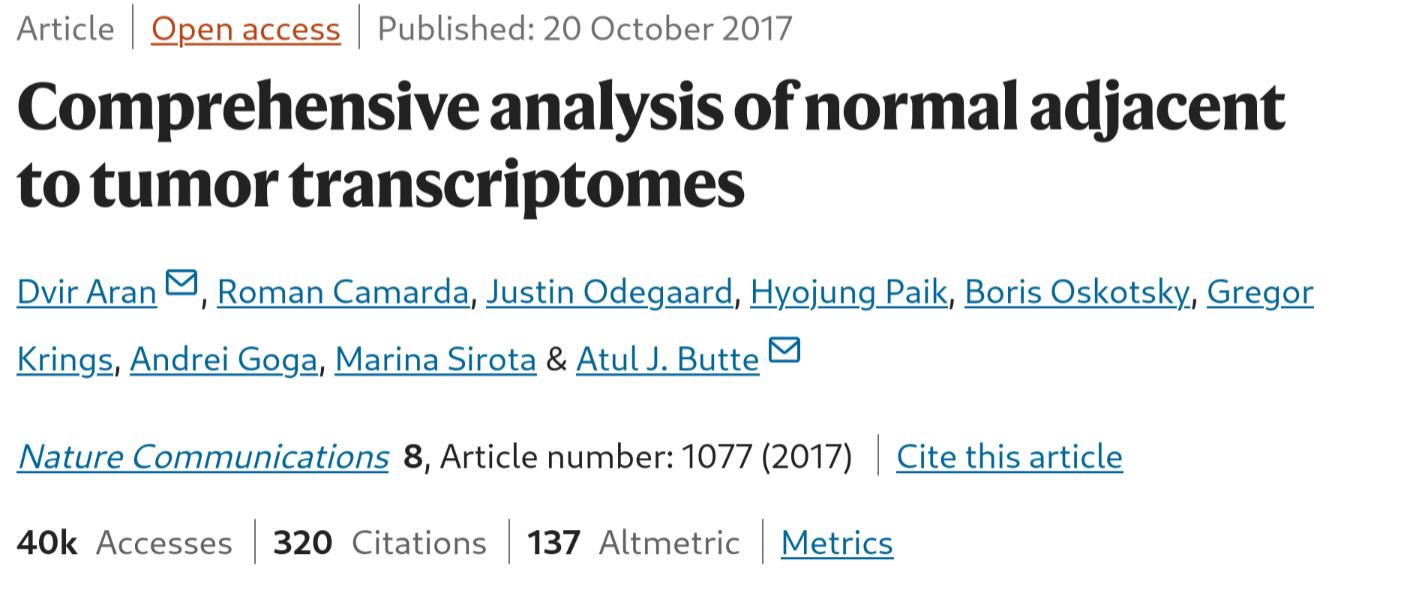
\includegraphics[scale=0.25]{/home/hh/data/output/paper_image.png}
  \end{center}
  
\end{frame}

\begin{frame}
  \frametitle{Example Experiment}
   \begin{columns}
     \begin{column}{0.5\textwidth}
      \begin{center}
        \underline{Healthy}
        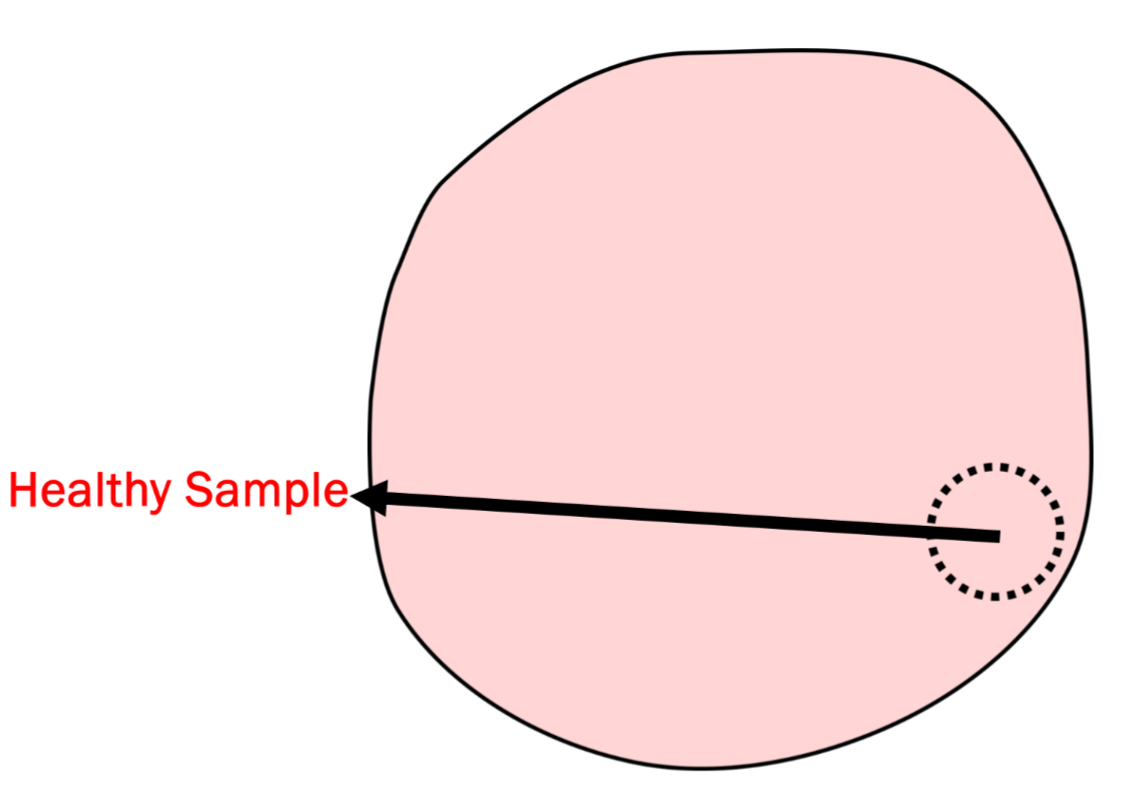
\includegraphics[scale=0.16]{/home/hh/data/output/healthy.png}
      \end{center}
    \end{column}
    \vrule{}
    \begin{column}{0.5\textwidth}  %%<--- here
      \begin{center}
        \underline{Normal-Adjacent-to-Tumor (NAT)}
        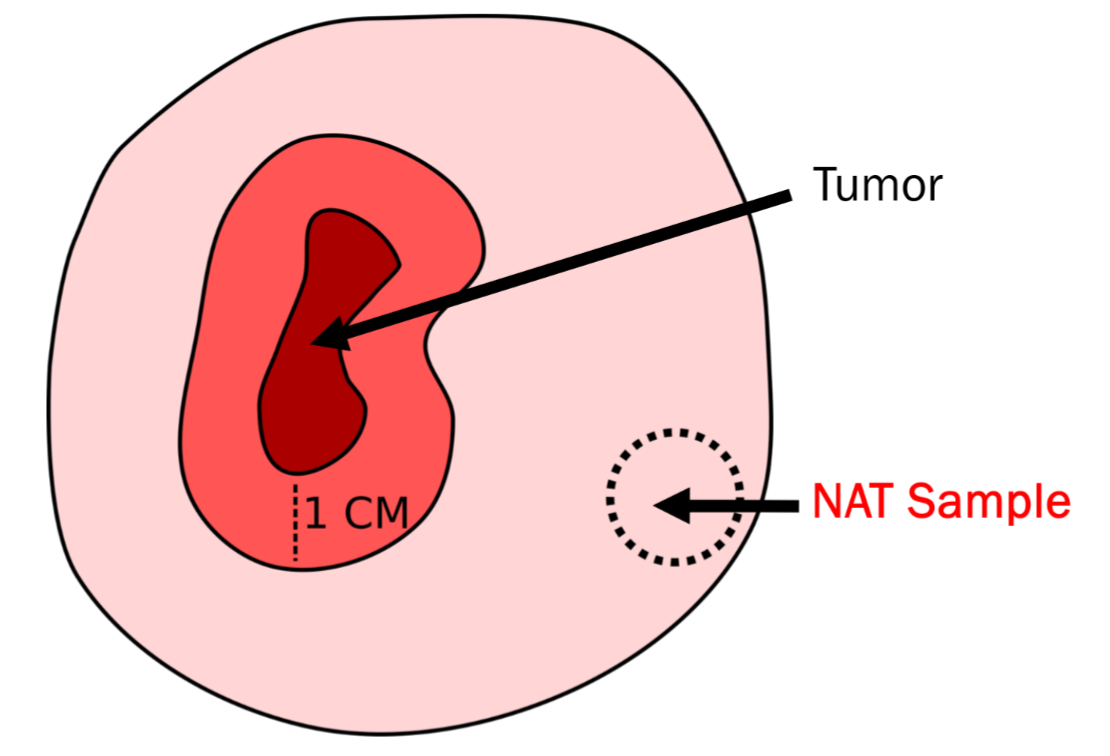
\includegraphics[scale=0.16]{/home/hh/data/output/nat.png}
      \end{center}
    \end{column}
   \end{columns}
   \begin{exampleblock}{Research Question}
     Is NAT tissue an appropriate proxy for healthy tissue in cancer research?
   \end{exampleblock}
\end{frame}

\begin{frame}
  \frametitle{Example Experiment}
  \begin{center}
    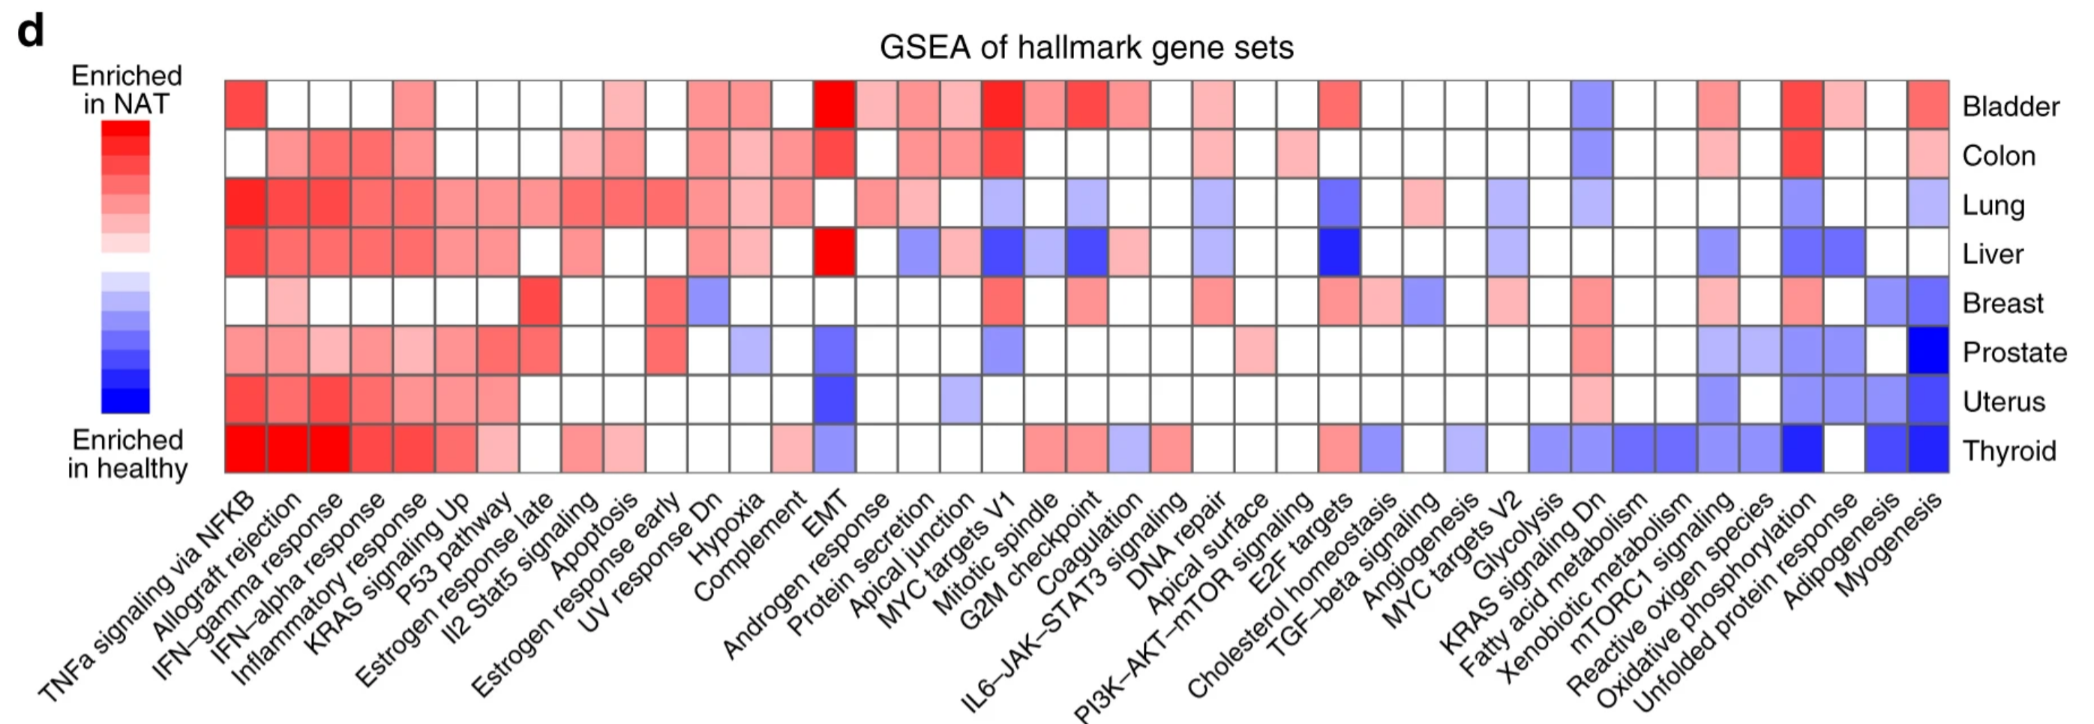
\includegraphics[scale=0.16]{/home/hh/data/output/aran_res.png}
  \end{center}
  \begin{exampleblock}{Key Points about Pathway Enrichment Results}
    \begin{enumerate}
      \item Inflammatory-related pathways enriched in NAT (e.g., TNF-\(\alpha\) signaling and interferon response)
      \item Metabolic/Differentiation pathways enriched in healthy (e.g., Myogenesis)
    \end{enumerate}
  \end{exampleblock}
\end{frame}

\begin{frame}
  Exploring how error in scale (normalization) assumptions affect these results
\end{frame}
  
\begin{frame}
  \frametitle{The GSEA Algorithm}
  \begin{center}
    \includegraphics[scale=0.28]{/home/hh/data/output/gsea_paper.png}
  \end{center}  
\end{frame}

\begin{frame}
  \frametitle{Key Points about the GSEA Algorithm}
  \begin{enumerate}
    \item GSEA's input is estimated LFCs \(\hat{\theta}\) and a gene/microbe set \(S\)
      \begin{itemize}
        \item e.g., \(S=\{\text{EGFR},\text{B2M}, \dots, \text{RAD1}\}\)
      \end{itemize}
    \item GSEA returns an Enrichment Score (ES) (i.e., effect size) and p-value
    \item GSEA uses a weighting schema that \textbf{depends on } \(\hat{\theta}\):
      \begin{itemize}
        \item Changes to \(\hat{\theta}\) affect the ES / p-value
      \end{itemize}
    \item GSEA is a permutation test using gene label permutations:
      \underline{Original Gene Set}
      
      \begin{align*}
        S=\{\text{EGFR},\text{B2M}, \dots, \text{RAD1}\}
      \end{align*}
      
        \underline{Permuted Gene Sets}
        \begin{align*}
          S^*_1&=\{\text{EGFR},\text{B2M}, \dots, \text{RAD1}\} \\
          S^*_2&=\{\text{EGFR},\text{B2M}, \dots, \text{RAD1}\}
        \end{align*}
        
  \end{enumerate}
\end{frame}

\begin{frame}
  \frametitle{GSEA with Gene Label Permutations}

  The GSEA algorithm proposed by Subramanian et al. involves X key steps:
  \begin{enumerate}
    \item Pick Gene Set(s)
      \begin{itemize}
        \item e.g., \(S=\{\text{EGFR}, \text{B2M}, \dots, \text{MTOR}\}\)
      \end{itemize}
    \item Estimate LFCs \(\hat{\theta}=f(Y)\)
      \begin{itemize}
        \item e.g., with DESeq2, limma, ALDEx2, Songbird, etc.
      \end{itemize}
    \item Rank the genes in descending order by LFC
    \item \textbf{Weight the genes by their LFC}
    \item Calculate a Running Sum, Enrichment Score, and p-value
  \end{enumerate}
\end{frame}

\begin{frame}
  \frametitle{GSEA with Gene Label Permutations}

  Mathematically the GSEA Algorithm can be written as a function \(g\):
  \begin{align*}
    g(\hat{\theta}, S) = (\text{ES}, p)
  \end{align*}

  \vspace{5px}

  What about scale error \(\epsilon^\perp\)?

  \vspace{10px}
  \begin{align*}
    \underbrace{\theta^\perp}_{\text{True LFC in Scale}} = \underbrace{\hat{\theta}^\perp}_{\text{Estimated LFC in Scale}} + \underbrace{\epsilon^\perp}_{\text{Scale Estimation Error}}
  \end{align*}
\end{frame}

\begin{frame}
  \frametitle{Frequentist LFC Sensitivity Analysis}
  \begin{align*}
    \underbrace{\theta^\perp}_{\text{True LFC in Scale}} = \underbrace{\hat{\theta}^\perp}_{\text{Estimated LFC in Scale}} + \underbrace{\epsilon^\perp}_{\text{Scale Estimation Error}}
  \end{align*}

  If we assume little compositional error (\(\theta^\parallel \approx \hat{\theta}^\parallel\)):
  \begin{align*}
    \underbrace{\theta_d}_{\text{True LFC}} &\approx \underbrace{\hat{\theta}^\parallel_d}_{\text{Estimated LFC in Composition}} + \underbrace{\hat{\theta}^\perp}_{\text{Estimated LFC in Scale}} + \underbrace{\epsilon^\perp}_{\text{Scale Estimation Error}} \\
                                        &\approx \underbrace{\theta_d}_{\text{Estimated LFC}} + \underbrace{\epsilon^\perp}_{\text{Scale Estimation Error}}
  \end{align*}
\end{frame}

\begin{frame}
  \frametitle{Frequentist LFC Senstivity Analysis}
  \begin{align*}
    \underbrace{\theta_d}_{\text{True LFC}} \approx \underbrace{\theta_d}_{\text{Estimated LFC}} + \underbrace{\epsilon^\perp}_{\text{Scale Estimation Error}}
  \end{align*}

  \underline{Frequentist LFC Sensitivity Analysis}
  \begin{align*}
    g(\hat{\theta}+\epsilon^\perp, S) = (\text{ES}, p)
  \end{align*}

  \textbf{All we need to do is rerun GSEA for different \(\epsilon^\perp\) and visualize how Enrichment Score (ES) and p-value changes}
  
\end{frame}

\begin{frame}
  \frametitle{Frequentist LFC Senstivity Analysis: A Simulation}

  \begin{center}
    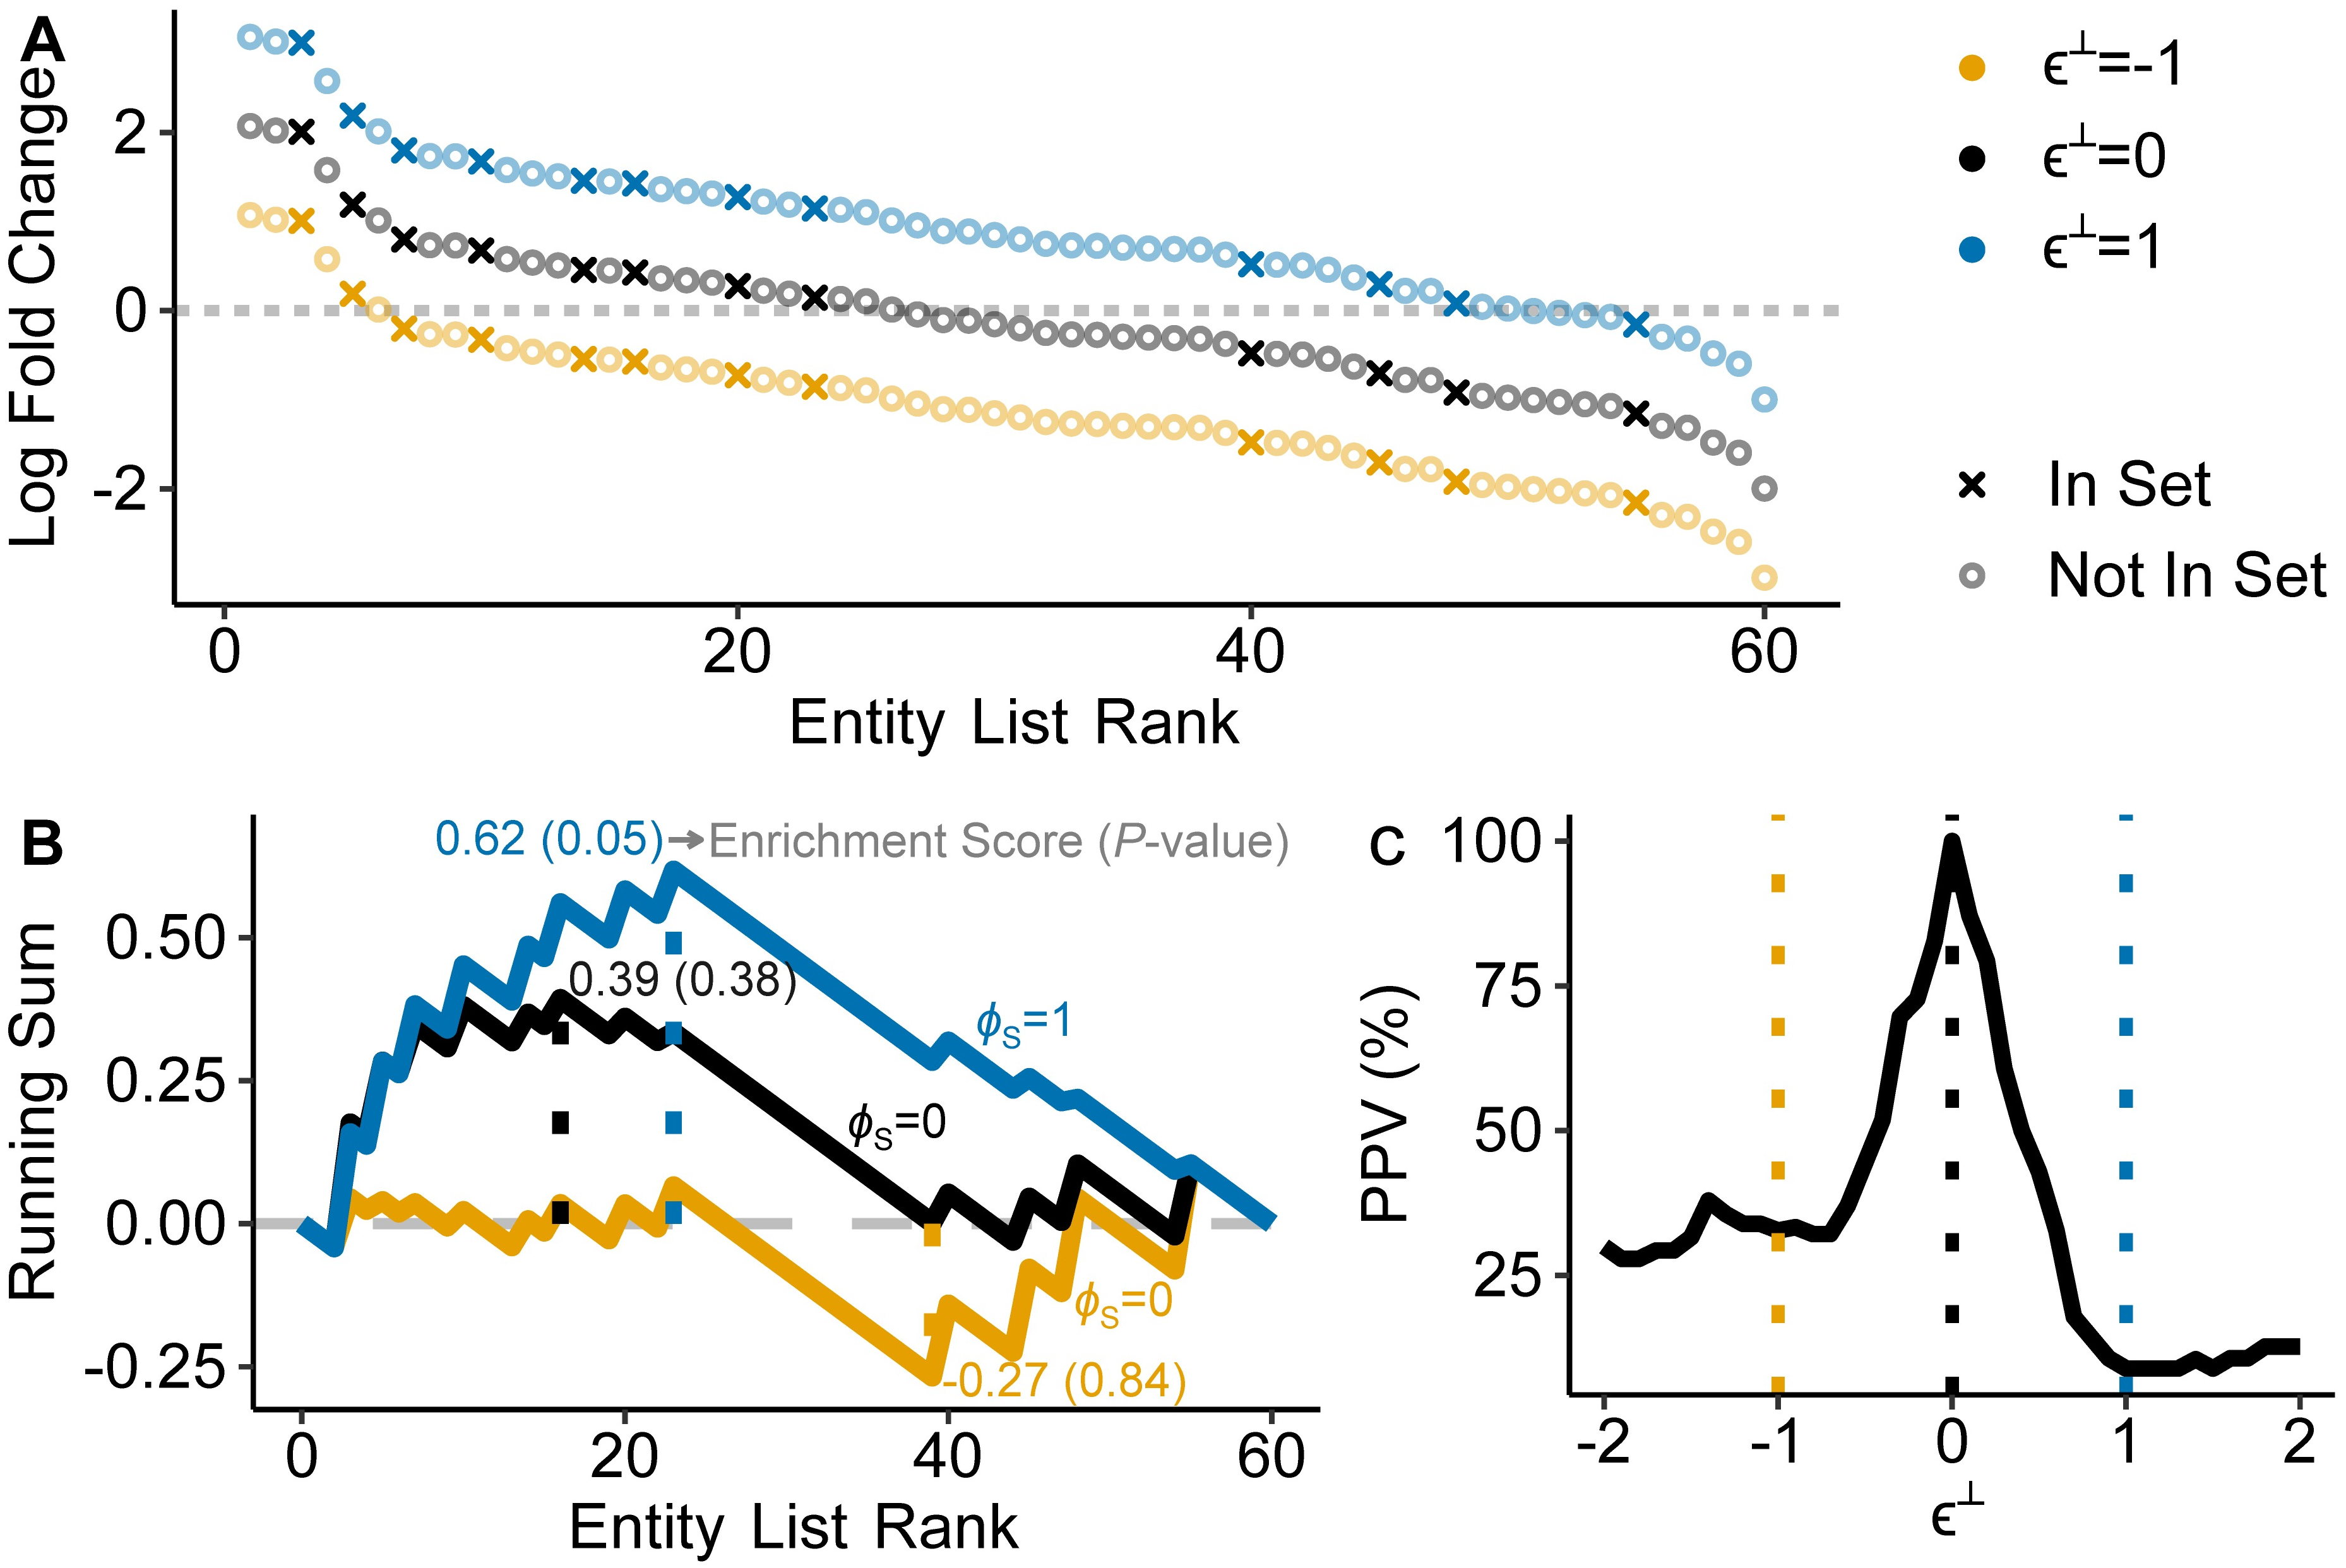
\includegraphics[scale=0.7]{/home/hh/data/output/first_fig.png}
  \end{center}
\end{frame}

\begin{frame}
  \frametitle{Returning to NAT vs. Healthy Tissue}

  Aran et al. found:
  \begin{enumerate}
    \item Myogenesis is enriched in healthy thyroid tissue
    \item INF-\(\gamma\) is enriched in NAT thyroid tissue
  \end{enumerate}
  
  Results using the fast GSEA (fgsea) package:
  \begin{center}
    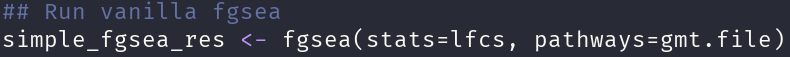
\includegraphics[scale=0.4]{/home/hh/data/output/vanilla_fgsea.png}
  \end{center}
  \begin{columns}
    \begin{column}{0.5\textwidth}
      \begin{center}
        \underline{Myogenesis}
        
        \begin{tabular}{ |c|c| } 
        \hline
        adj. p-value & \textbf{9e-9} \\
        \hline
        NES & -2.1 \\
        \hline
        \end{tabular}
      \end{center}
    \end{column}
    \vrule{}
    \begin{column}{0.5\textwidth}  %%<--- here
      \begin{center}
        \underline{Inflamatory Response}
        
        \begin{tabular}{ |c|c| } 
        \hline
        adj. p-value & \textbf{3e-3} \\
        \hline
        NES & 1.5 \\
        \hline
        \end{tabular}
      \end{center}
    \end{column}
   \end{columns}
\end{frame}

\begin{frame}
  \frametitle{Returning to NAT vs. Healthy Tissue}
  
  Results using the fast GSEA (fgsea) package:
  \begin{columns}
    \begin{column}{0.5\textwidth}
      \begin{center}
        \underline{Myogenesis}
        
        \begin{tabular}{ |c|c| } 
        \hline
        adj. p-val & \textbf{9e-9} \\
        \hline
        NES & -2.1 \\
        \hline
        \end{tabular}
      \end{center}
    \end{column}
    \vrule{}
    \begin{column}{0.5\textwidth}  %%<--- here
      \begin{center}
        \underline{Inflamatory Response}
        
        \begin{tabular}{ |c|c| } 
        \hline
        adj. p-val & \textbf{3e-3} \\
        \hline
        NES & 1.5 \\
        \hline
        \end{tabular}
      \end{center}
    \end{column}
   \end{columns}

  \vspace{10px}
  Results using fgsea \textbf{LFC Sensitivity Analysis} wrapper:
  \begin{center}
    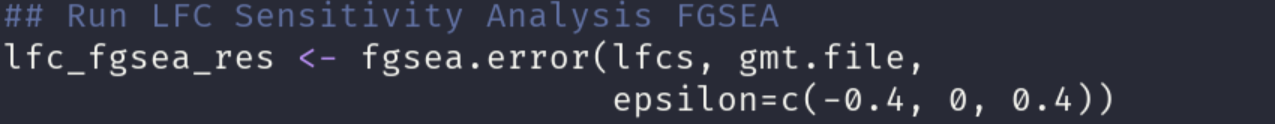
\includegraphics[scale=0.25]{/home/hh/data/output/lfc_sens.png}
  \end{center}
  \begin{columns}
    \begin{column}{0.5\textwidth}
      \begin{center}
        \begin{tabular}{ |c|c|c|c| } 
        \hline
        \(\epsilon^\perp\) & \(-0.4\) & \(0\) & \(0.5\) \\
        \hline
        adj. p-val & \textbf{2e-6} & \textbf{9e-9} & \textbf{2e-9} \\
        \hline
        NES & -1.4 & -2.1 & -2.5 \\
        \hline
        \end{tabular}
      \end{center}
    \end{column}
    \vrule{}
    \begin{column}{0.5\textwidth}  %%<--- here
      \begin{center}
        \begin{tabular}{ |c|>{\columncolor{gray}}c|c|c| } 
        \hline
        \(\epsilon^\perp\) & \(-0.4\) & \(0\) & \(0.5\) \\
        \hline
        adj. p-val & 1 & \textbf{3e-3} & \textbf{3e-3} \\
        \hline
        NES & -0.8 & 1.5 & 1.6 \\
        \hline
        \end{tabular}
      \end{center}
    \end{column}
   \end{columns}
\end{frame}

\begin{frame}
  \frametitle{Returning to NAT vs. Healthy Tissue}

  Aran et al.'s original results for Thyroid tissue
  \begin{center}
    \includegraphics[scale=0.17]{/home/hh/data/output/thyroid.png}
  \end{center}
\end{frame}
  
\begin{frame}
  \frametitle{Thyroid NAT vs Healthy LFC Sensitivity Analysis}
   \begin{center}
    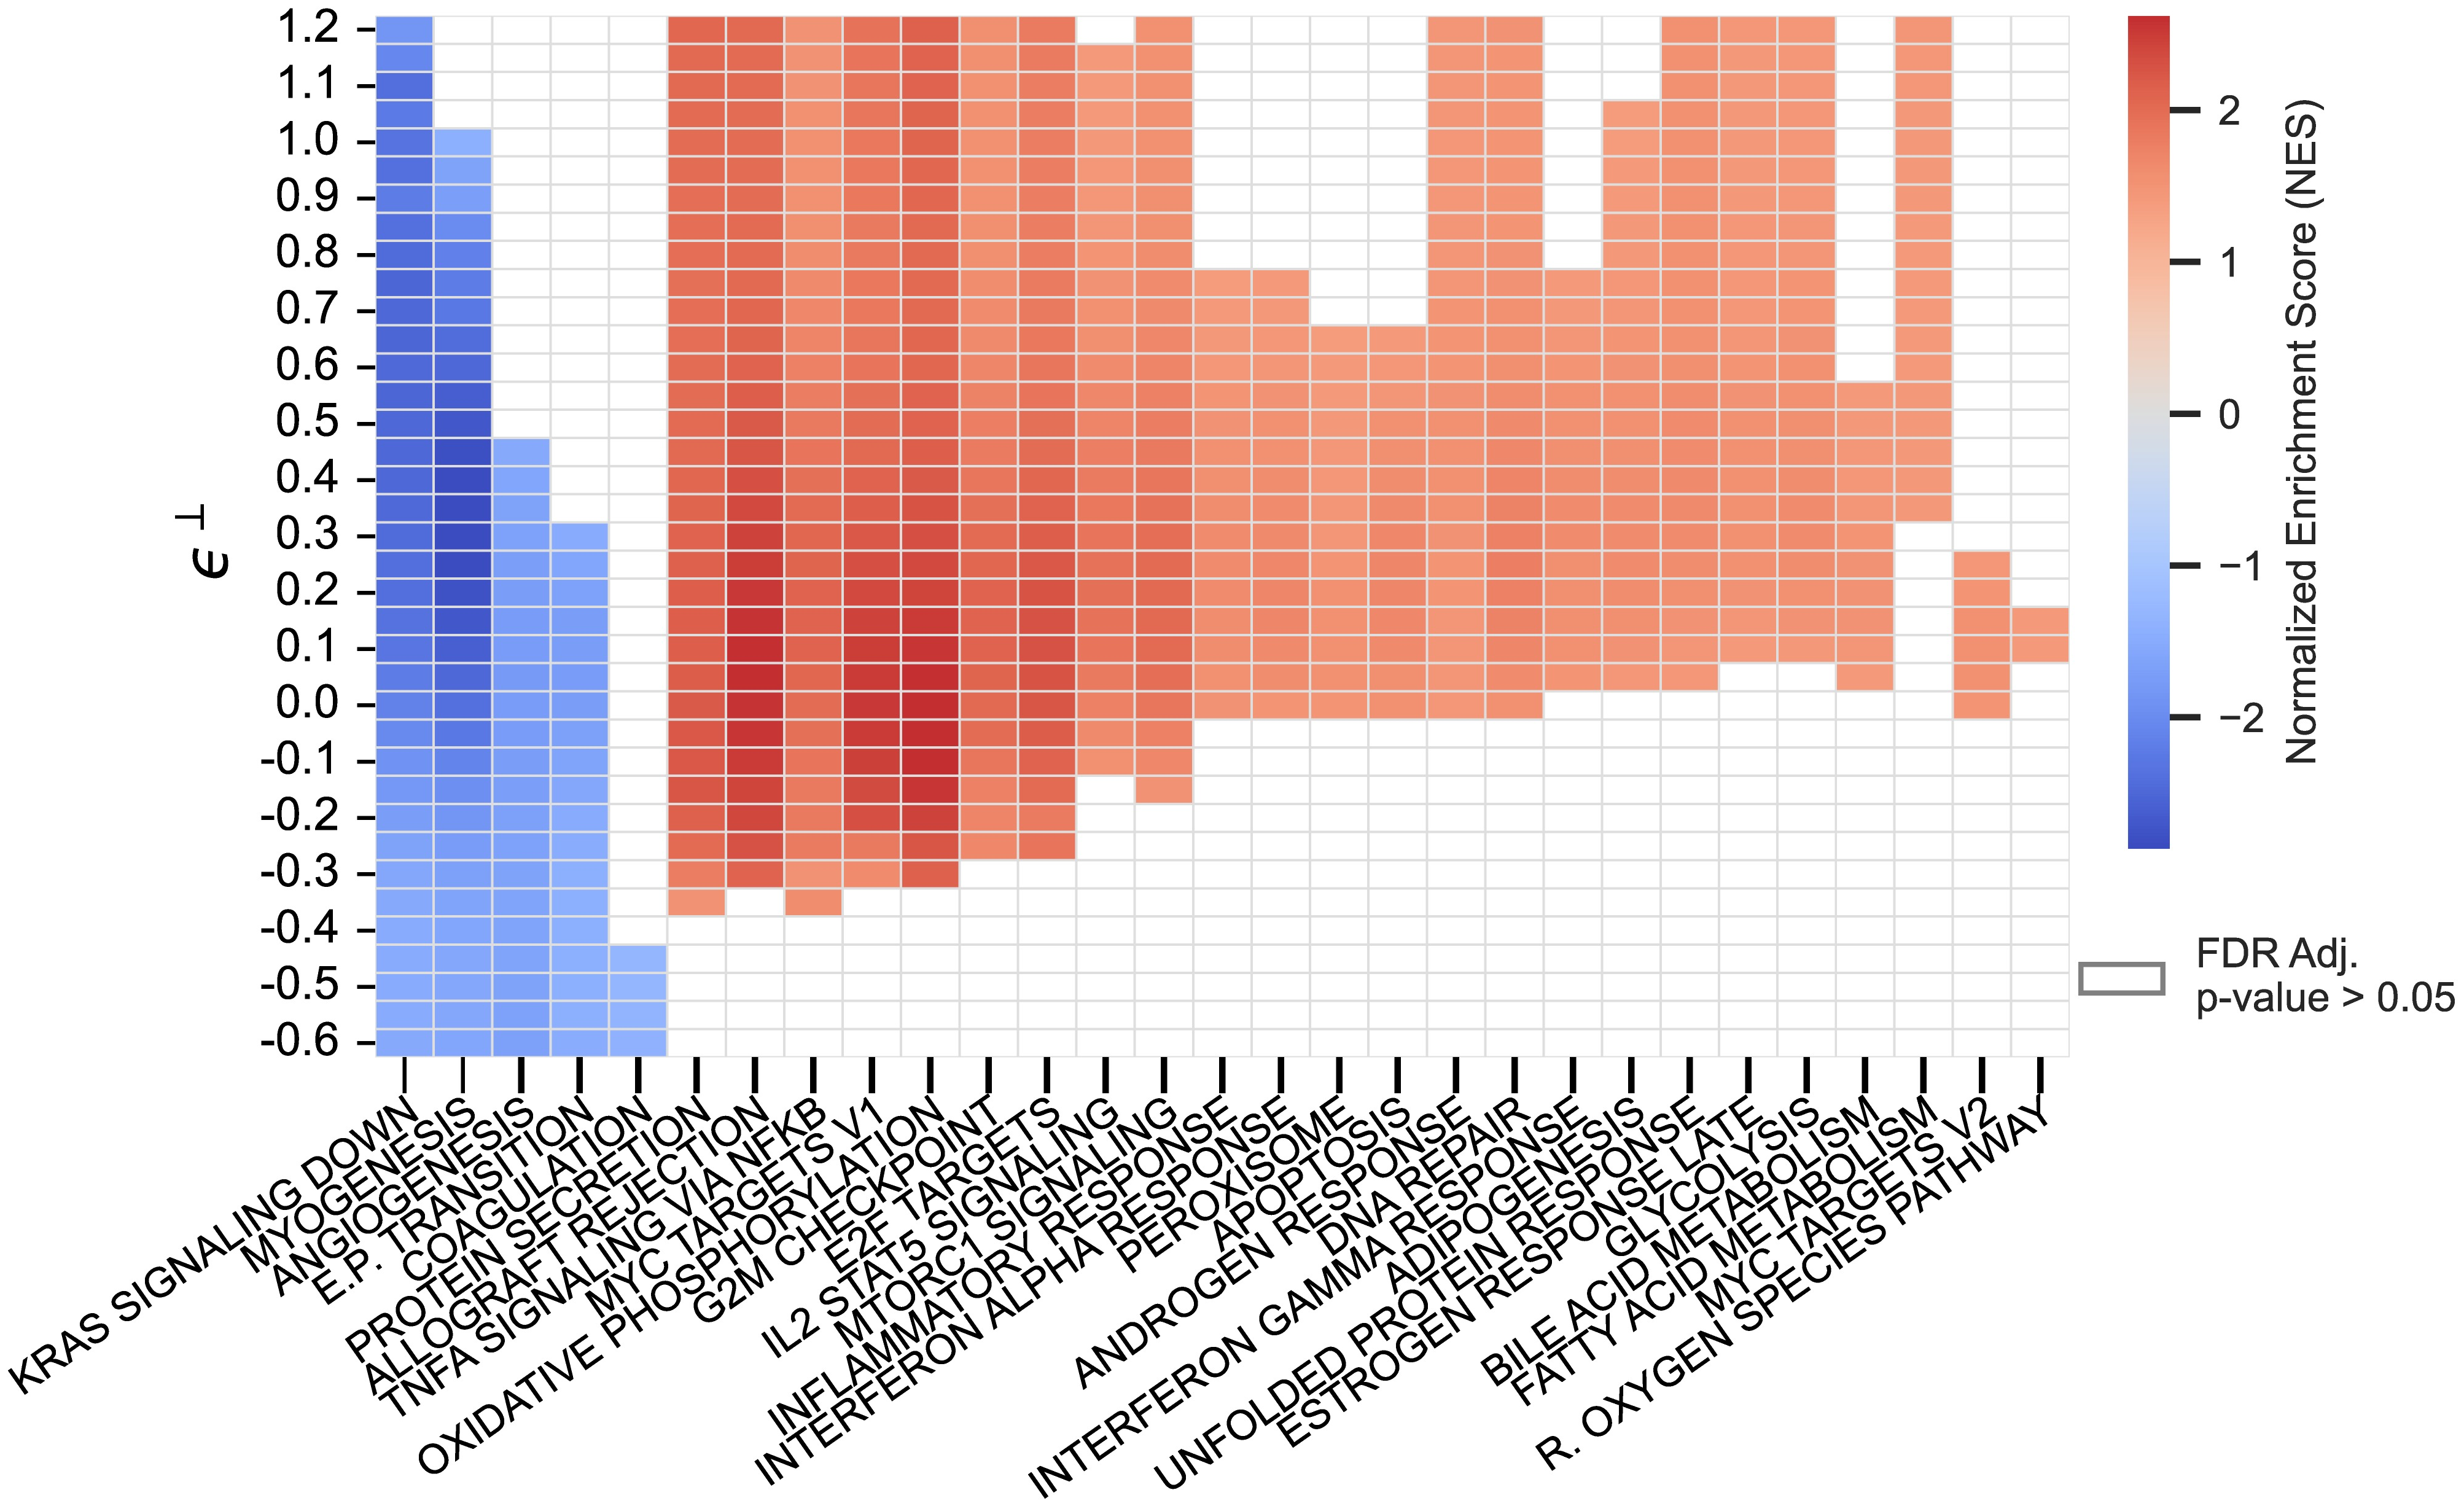
\includegraphics[scale=0.7]{/home/hh/data/output/thyroid_lfc_sens.png}
  \end{center}
\end{frame}

\begin{frame}
  \frametitle{Frequentist LFC Sensitivity Testing}

  Let \(p_{\epsilon^\perp}\) be the GSEA p-value at \(\epsilon^\perp\), the \textbf{LFC Sensitivity Test}:
  \begin{align*}
    p = \sup_{\epsilon^\perp \in (-\infty, \infty)} p_{\epsilon}
  \end{align*}

  Remarkably this test has non-zero power:
  \begin{enumerate}
  \item Hallmark Gene Sets: 0 /50 Significant
  \item C2 Gene Sets: X/Y Significant
  \end{enumerate}

  \vspace{10px}
  \begin{block}{Improving Power of Test}
    Why consider all possible \(\epsilon^\perp \in (-\infty,\infty)\)? For instance \(\epsilon^\perp=10\) implies expression is 22,000 times higher in NAT than healthy tissue!
  \end{block}
\end{frame}

\begin{frame}
  \frametitle{a}
  Bayesian Approacj
\end{frame}

\end{document}
